%!TEX root = ../template.tex
%%%%%%%%%%%%%%%%%%%%%%%%%%%%%%%%%%%%%%%%%%%%%%%%%%%%%%%%%%%%%%%%%%%%
%% chapter2.tex
%% NOVA thesis document file
%%
%% Chapter with the template manual
%%%%%%%%%%%%%%%%%%%%%%%%%%%%%%%%%%%%%%%%%%%%%%%%%%%%%%%%%%%%%%%%%%%%

\typeout{NT FILE chapter2.tex}

\chapter{Digital Image Correlation}
\label{cha:digital_image_correlation}

\section{What is it?}
\label{sub:dic_definition}

% Compared to strain gages and extensometers, the amount of information gathered about the fine details of deformation during mechanical tests is increased due to the ability to provide both local and average data using digital image correlation.


%The tracking creates in-plane displacement patterns, from which strains are calculated. Multiple cameras triangulating on the points can map out-of-plane displacements as well. During the test, the movement of the spots are recorded digitally, and appropriate derivatives of displacement are taken to arrive at strains.



Digital image correlation, DIC, is an optical full-field strain measurement technique for 2D or 3D ANALYSIS. IN A SIMPLER MANNER OF SPEECH, DIC consists in the comparison of two images of an object before and after its deformation.\\
This technique has first been applied to digital images in 1975 and, thanks to the progress of technology and improvement of cameras, it has become a reliable technique for many present-day applications, like image analysis, velocimetry, and strain estimation.\\

Normally, in order to perform the technique, the sample surface is painted with a solid base colour, normally black or white, and then SPRINKLED/SPRAYED WITH A CONTRASTING COLOUR, creating distinct patterns all over it. Those patterns are then taken as reference in the control, non-deformed, picture, and compared, in terms of displacement and DEFORMATION, with the patterns of the following deformed pictures, from which the strains can also be calculated through.\\

This method of analysis is possible by transforming the pictures into matrices, where each of its units represent subsets or blocks of pixels, correlating the position of such pixels in the original and deformed pictures, as shown in the figure~\ref{fig:dic}, hence the need of creating distinct patterns. It also allows the \\

\begin{figure}[h!]
	\centering
	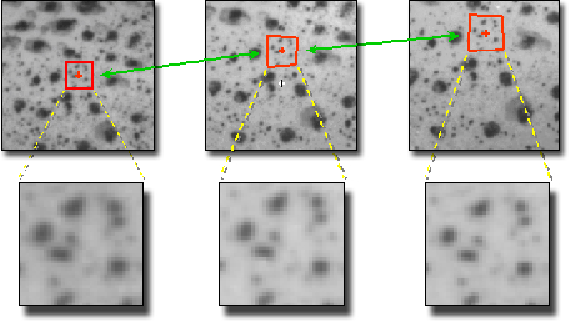
\includegraphics[scale=1]{DIC}
	\caption{Example of image correlation}
	\label{fig:dic}
\end{figure}


The developed software is a 2D DIC and 


%It is also possible to estimate shifts to a finer resolution than the resolution of the original images, which is often called "subpixel" registration because the measured shift is smaller than an integer pixel unit. 






% https://www.sciencedirect.com/topics/engineering/digital-image-correlation
% Donald F. Adams, Thomas J. Whitney, in Comprehensive Composite Materials II, 2018
% M.A. Rastak, Mahmood M. Shokrieh, L.Barrallier, R. Kubler, S.D. Salehi, in Residual Stresses in Composite Materials (Second Edition), 2021
% W. Broughton, in Adhesives in Marine Engineering, 2012
% https://en.wikipedia.org/wiki/Digital_image_correlation_and_tracking